% LTeX: language=en-GB
% !TEX root = ../../report.tex

\section{Step 3 - Sled test (FEM)}\label{section:step3-sledTest}
The scope of this third step within the workflow is to subject the payload bay, i.e. the container of the medical payload analysed until now, to the type of acceleration it would possibly undergo in an impact event. Specifically, the idea is to imitate a \textit{sled test}, which is common practice in the automotive industry: an ATD\footnote{\textit{Anthropomorphic Test Devices}.} crash dummy is strapped onto a sled (a trolley sliding on almost frictionless rails) that is subjected to a prescribed acceleration pulse, and the response of the dummies, governed predominantly by their own inertia and the forces exerted by the restraint system, is checked against damage thresholds \hl{cite that paper with the sled test and dummy damage indices!!!!} 

The model built in this Step 3 aims to simulate a similar phenomenon: here, an acceleration boundary condition is imposed on the external shell of the medical payload container, leaving its contents to be governed by their inertial response and by the contact forces exchanged between each other. The model aims to verify whether the imposed acceleration impulse damages the medical payload inside, i.e. the glass phials. The outcome is, therefore, binary: either the phials are damaged, or they are not. The information related to crack initiation and material failure is monitored through the same LS-DYNA variable activated in Step 2 to evaluate phial failure load under axial compression. The apparition of damage implies that the acceleration pulse to which the container was subjected was too high for the phials to resist and the \textit{allowable} (i.e. maximum withstandable) peak acceleration must correspond to a lower value. The test is in itself can be reduced to a threshold problem, where exceeding a certain peak acceleration immediately induces damage (with due considerations on tolerance). Finding the acceleration allowable $a_{allow}$ is an iterative process and results in obtaining the last input necessary for the airbag design optimisation code of the workflow's Step 4.

Just like the FEM model for the axial compression test, the present model is built using \textit{explicit} time integration with an engineering unit system consistent with the one adopted in Step 2, reported here again for clarity:
\begin{table}[htbp]
  \centering
  \caption{Engineering Units}
  \label{tab:units-Step3}
  \begin{thesistable}{
    colspec = {*{9}{X[c,m]}},
    colsep = 3pt,
  }
    Time & Distance & Mass & {Stress /\\Pressure} & Force & {Energy /\\Work}   & Velocity & Acceleration & Density \\
    ms   & mm       & kg   & {GPa\\(kN/mm$^2$)}   & kN    & {J\\(kN$\cdot$mm)} & mm/ms    & mm/ms$^2$         & kg/mm$^3$ \\
  \end{thesistable}
\end{table}

\subsection{Implementation}

\subsubsection{Model setup}
As illustrated in \cref{sec:reference-mission}, the payload container considered in this model is inspired by the designed proposed by Sivieri (2021) \cite{Sivieri2021}. The payload assembly presented here is composed of four parts, as shown in \cref{fig:payload-assembly}: the \textit{payload bay} (the outer shell of the receptacle), the \textit{sponge} (an internal buffer between the medical payload and the receptacle, conceptually representing a protective layer such as bubble wrap, of the kind an operator would use to attenuate in-flight vibrations), the medicinal \textit{mask} (a plastic tray commonly found in pharmaceutical packaging to hold the phials in place during transport), and the glass phials (as modelled in previous Step 2, and only including one in the model setup for exemplification), overall representing a realistic carry-on configuration for typical mission scenarios.

\begin{figure}[h!]
    \centering
    % TODO: replace the placeholder box with the actual figure once available
    % \includegraphics[width=0.8\textwidth]{figures/chap4/step3-sled/payload_assembly.png}
    \fbox{\parbox[c][6cm][c]{0.8\textwidth}{\centering Figure placeholder: payload assembly FEM model}}
    \caption{FEM model of the payload assembly, composed of the \textit{payload bay}, the \textit{sponge}, the \textit{mask} and the \textit{glass phials}.}
    \label{fig:payload-assembly}
\end{figure}

Two considerations should be made regarding the modelling choices:
\begin{enumerate}
    \item The presence of the sponge layer strongly affects the value of $a_{allow}$ as it heavily contributes to the attenuation mechanism protecting the phials. Therefore, to capture an accurate response, it is key to study the phials' behaviour in relation to their interaction with the assembly they belong to. The consequences of using a sponge in this context are explored in the following paragraphs;
    \item Apart from the phials' glass, only the payload bay's material has a failure criterion implemented, wrongly assuming that the sponge and the mask remain intact during an impact event. This non-realistic choice was made to purposefully focus on the accurate modelling of the phials' behaviour, supported by concrete experimental data. The other materials' data on mechanical properties is extracted from an ad-hoc literature review.
\end{enumerate}

The outer shell of the payload bay is meshed with shell elements of average length of 6\,mm size and 5\,mm thickness, default {ELFORM = 2} with two integration points through the thickness. Its material is injection-moulded ABS, modelled with \kw{MAT\_PIECEWISE\_LINEAR\_PLASTICITY} (material model \kw{MAT\_024}), as shown in \cref{lst:mat-bay}.

\begin{dynacard}[label=lst:mat-bay]{ABS material card for the payload bay}
*MAT_PIECEWISE_LINEAR_PLASTICITY
$HMNAME MATERIAL         2ABS_inject-mould
$---+----1----+----2----+----3----+----4----+----5----+----6----+----7----+----8
$      MID       RHO         E        PR      SIGY      ETAN      FAIL      TDEL
         2 1.050E-06      2.10      0.38     0.040     0.150     0.025
$        C         P      LCSS      LCSR        VP       LCF

$     EPS1      EPS2      EPS3      EPS4      EPS5      EPS6      EPS7      EPS8

$      ES1       ES2       ES3       ES4       ES5       ES6       ES7       ES8

\end{dynacard}

\noindent where the parameters set in the material card, taken from \hl{PUT A SOURCE HERE} are:

\begin{itemize}
  \item \texttt{RHO}: Density, 1.05E-06 kg/mm$^3$ (1050 kg/m$^3$);
  \item \texttt{E}: Young's modulus, 2.10\,GPa;
  \item \texttt{PR}: Poisson's ratio, 0.38;
  \item \texttt{SIGY}: Yield stress, 0.040\,GPa (40\,MPa);
  \item \texttt{ETAN}: Tangent modulus, 0.150\,GPa (150\,MPa), defining the slope of the hardening branch after yield. As no stress-strain curve is given (\texttt{LCSS} left blank), the material follows a bilinear elastic-plastic law;
  \item \texttt{FAIL}: Effective plastic strain at failure, 0.025, beyond which the element is deleted.
\end{itemize}


The mask holding the glass phials is meshed with shell elements of 0.5\,mm thickness, with the material card in \cref{lst:mat-mask}. The mask material is polypropylene (PP), modelled as linear elastic with \kw{MAT\_ELASTIC} (material model \kw{MAT\_001}), as shown in \cref{lst:mat-mask}. No failure criterion is defined, so the mask cannot fail.

\begin{dynacard}[label=lst:mat-mask]{PP material card for the mask}
*MAT_ELASTIC
$HMNAME MATERIAL         3polypropylene_PP
$HWCOLOR MATERIAL         3      25
$---+----1----+----2----+----3----+----4----+----5----+----6----+----7----+----8
$      MID       RHO         E        PR        DA        DB         K
         3 9.1000E-7     1.350       0.4
\end{dynacard}

\noindent where the parameters set in the material card, taken from \hl{PUT THE SOURCE HERE} are:

\begin{itemize}
  \item \texttt{RHO}: Density, 9.10E-07 kg/mm $^3$ (910 kg/m$^3$);
  \item \texttt{E}: Young's modulus, 1.35\,GPa;
  \item \texttt{PR}: Poisson's ratio, 0.40.
\end{itemize}

The sponge is meshed with [element type and size?]. Its loading curve was built to describe the typical behaviour of a porous foam: an initial soft branch, followed by hardening as the porosity closes and the material densifies. The curve is based on \hl{FIND SOURCE HERE} and is shown in \cref{fig:sponge_curve}, with the material card in \cref{lst:mat-sponge}.

The sponge material is a polyurethane foam, modelled with \kw{MAT\_LOW\_DENSITY\_FOAM} (material model \kw{MAT\_057}), as shown in \cref{lst:mat-sponge}.

\begin{dynacard}[label=lst:mat-sponge]{Polyurethane foam material card for the sponge}
*MAT_LOW_DENSITY_FOAM
$HMNAME MATERIAL         1polyurethane_foam
$---+----1----+----2----+----3----+----4----+----5----+----6----+----7----+----8
$      MID       RHO         E      LCID        TC        HU      BETA      DAMP
         1 2.500E-08       5.0         1                 1.0                0.05
$    SHAPE      FAIL    BVFLAG        ED     BETA1      KCON       REF

\end{dynacard}

\noindent where the parameters set in the material card, taken from \hl{PUT A SOURCE HERE} are:

\begin{itemize}
  \item \texttt{RHO}: Density, 2.50E-08 kg/mm$^3$ (25 kg/m$^3$);
  \item \texttt{E}: Young's modulus \hl{recheck the manual} used in tension, 5.0\,GPa;
  \item \texttt{LCID}: ID of the load curve defining the nominal stress versus strain in compression, i.e. curve 1, given in \cref{lst:curve-sponge} and plotted in \cref{fig:sponge_curve};
  \item \texttt{HU}: Hysteretic unloading factor, 1.0. With this value there is no hysteretic unloading: the foam unloads along the loading curve and no energy is dissipated through hysteresis;
  \item \texttt{DAMP}: Viscous coefficient, 0.05, which models damping effects (recommended range 0.05-0.50 according to the LS-DYNA user manual \hl{FIND EXACT PAGES}).
\end{itemize}

\begin{figure}[htbp]
  \centering
  \begin{minipage}[c]{0.52\textwidth}
    \renewcommand{\dynafont}{\scriptsize}
    \begin{dynacard}[label=lst:curve-sponge]{Sponge loading curve}
*DEFINE_CURVE_TITLE
$HMCURVE     1    2 polyurethane_curve
$NAME
polyurethane_curve
$     LCID      SIDR       SFA       SFO      OFFA      OFFO
         1                 1.0       1.0
$                  X                   Y
                 0.0                 0.0
                0.05             3.0E-06
                 0.1             5.0E-06
                 0.2             6.0E-06
                 0.4             7.0E-06
                 0.6             9.0E-06
                 0.7             1.5E-05
                 0.8             4.0E-05
                 0.9             1.5E-04
    \end{dynacard}
  \end{minipage}\hfill
  \begin{minipage}[c]{0.45\textwidth}
    \centering
    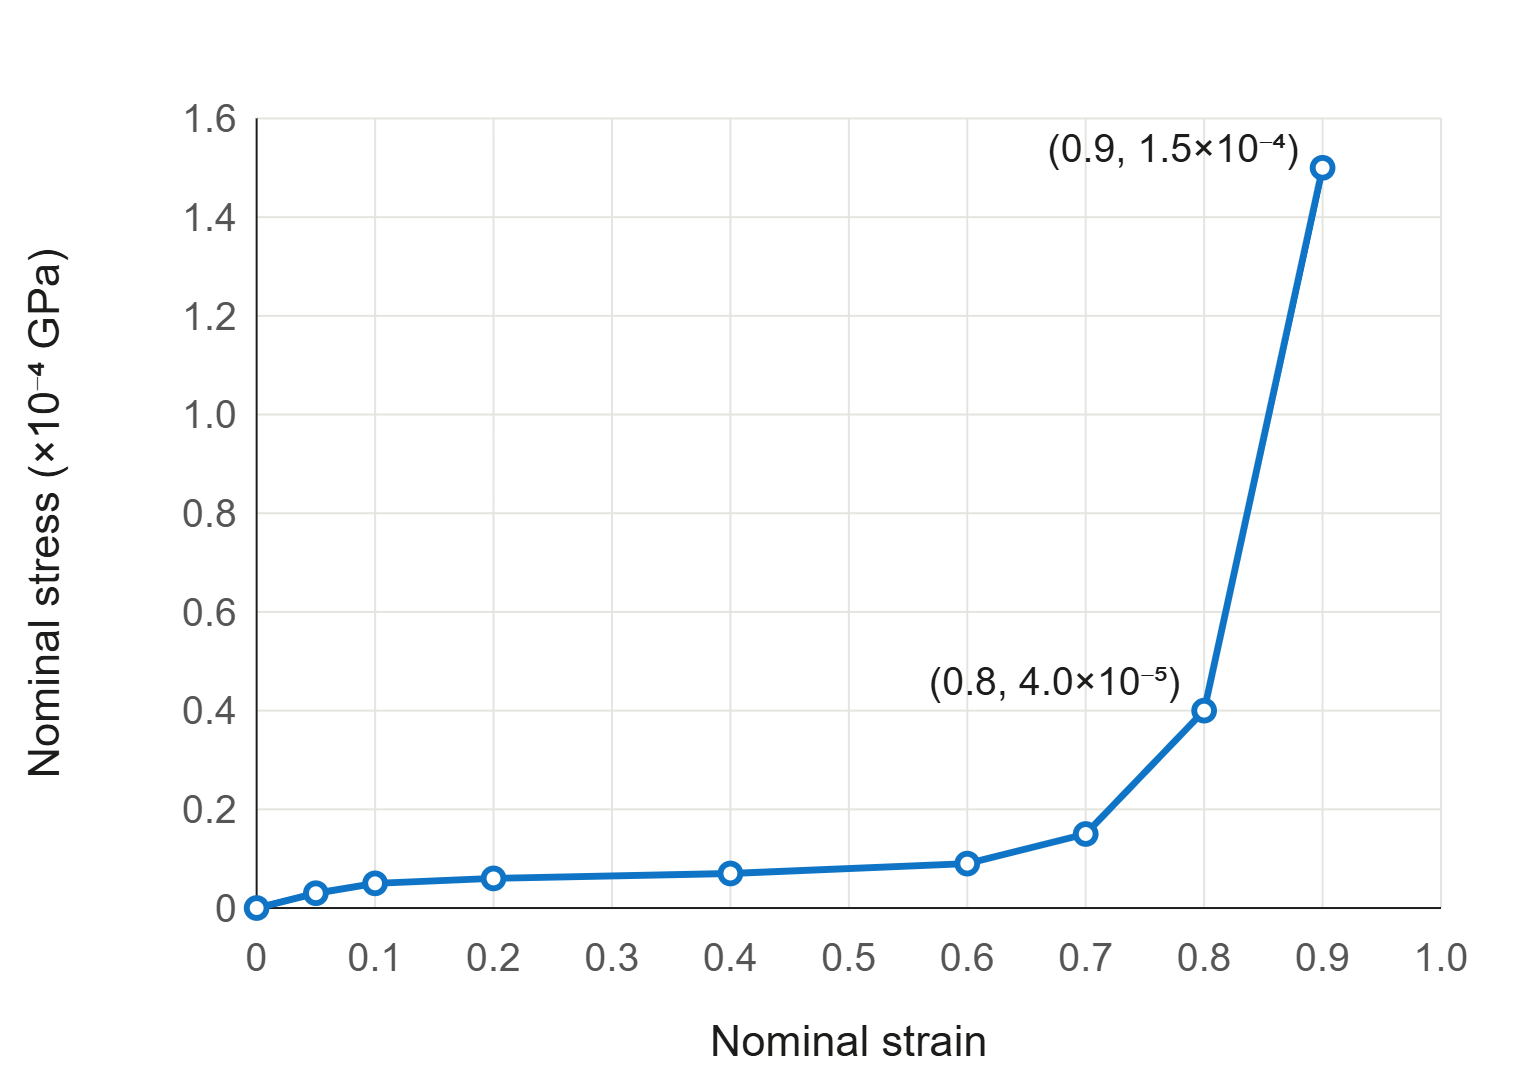
\includegraphics[width=\linewidth]{figures/chap4/step3-fem-sled/Polyurethane-curve.png}
    \caption{Nominal stress-strain loading curve of the polyurethane sponge.}
    \label{fig:sponge_curve}
  \end{minipage}
\end{figure}

The parts interact through \kw{CONTACT\_AUTOMATIC\_GENERAL} in LS-DYNA, which again treats every part as potentially in contact with every other part without master-slave couples hierarchy. In addition, an interior contact option was activated through the \kw{CONTACT\_INTERIOR} keyword to prevent negative volume formation during large compression events.



\subsubsection{Loading through an acceleration pulse}
The displacement forced onto the payload bay is applied through an acceleration pulse prescribed through \kw{BOUNDARY\_PRESCRIBED\_MOTION\_RIGID} on a selection of nodes on the bay's mesh forming two rigid rings through the keyword \kw{CONSTRAINED\_NODAL\_RIGID\_BODY} (see \cref{fig:rigid-rings}), virtually representing the strapping mechanism that would be implemented in the corresponding laboratory sled test. The rest of the bay remains deformable. The prescribed acceleration-time curve has a trapezoidal shape: an initial ramp of duration $t_r$, a plateau at constant acceleration $a$ of duration $t_p$, and a descending ramp of duration $t_r$ again\footnote{The duration of $t_r$ with respect to the entire duration of the phenomenon is governed by the parameter \texttt{RISE\_FRACTION}~$\in (0,\,0.5)$ that is arbitrarily set to 0.2 to generate the present family of curves. A value of \texttt{RISE\_FRACTION = 0} implies a fully rectangular pulse, while \texttt{RISE\_FRACTION = 0.5} corresponds to a triangular-shaped pulse.}. The ramps avoid discontinuities in the acceleration, which would excite spurious high-frequency oscillations, so that the velocity and displacement histories remain smooth. The acceleration is therefore applied at the attachment points, with the possibility to choose the degree of freedom in which to displace the bay (namely X, Y, or Z, and sweeping to detect the most critical one), and reaches the phials only after being transmitted through the deformable bay, the sponge and the mask.

\begin{figure}[h!]
    \centering
    % TODO: replace the placeholder box with the actual figure once available
    % \includegraphics[width=0.8\textwidth]{figures/chap4/step3-fem-sled/rigid_rings.png}
    \fbox{\parbox[c][6cm][c]{0.8\textwidth}{\centering Figure placeholder: rigid rings on the payload bay mesh}}
    \caption[Rigid rings on the payload bay mesh]{Nodes of the payload bay mesh constrained through \kw{CONSTRAINED\_NODAL\_RIGID\_BODY} into two rigid rings, onto which the acceleration pulse is prescribed.}
    \label{fig:rigid-rings}
\end{figure}

The impact is characterised by an initial velocity $\mathbf{u}_0 = (u_{x0}, u_{y0})$, which includes both horizontal and vertical components. Over the deceleration process, this velocity must be brought completely to zero. Therefore, the integral of the acceleration curve described above must equal the velocity shed by the system:
\begin{equation}
  \int_0^{T} a(t)\,\mathrm{d}t = a\,(t_r + t_p) = \lVert \mathbf{u}_0 \rVert,
  \qquad T = 2t_r + t_p .
  \label{eq:pulse_area}
\end{equation}

This condition allows to define a family of acceleration curves as shown in \cref{fig:accel-pulses}: for a given amplitude $a$, \cref{eq:pulse_area} fixes the plateau duration $t_p = \lVert \mathbf{u}_0 \rVert / a - t_r$, and therefore the characteristic time scale of the event. The aim is to reproduce the pulse felt by the payload bay during an impact as closely as possible, applying an acceleration profile similar to the peak observed in such an event.

\begin{figure}[h!]
    \centering
    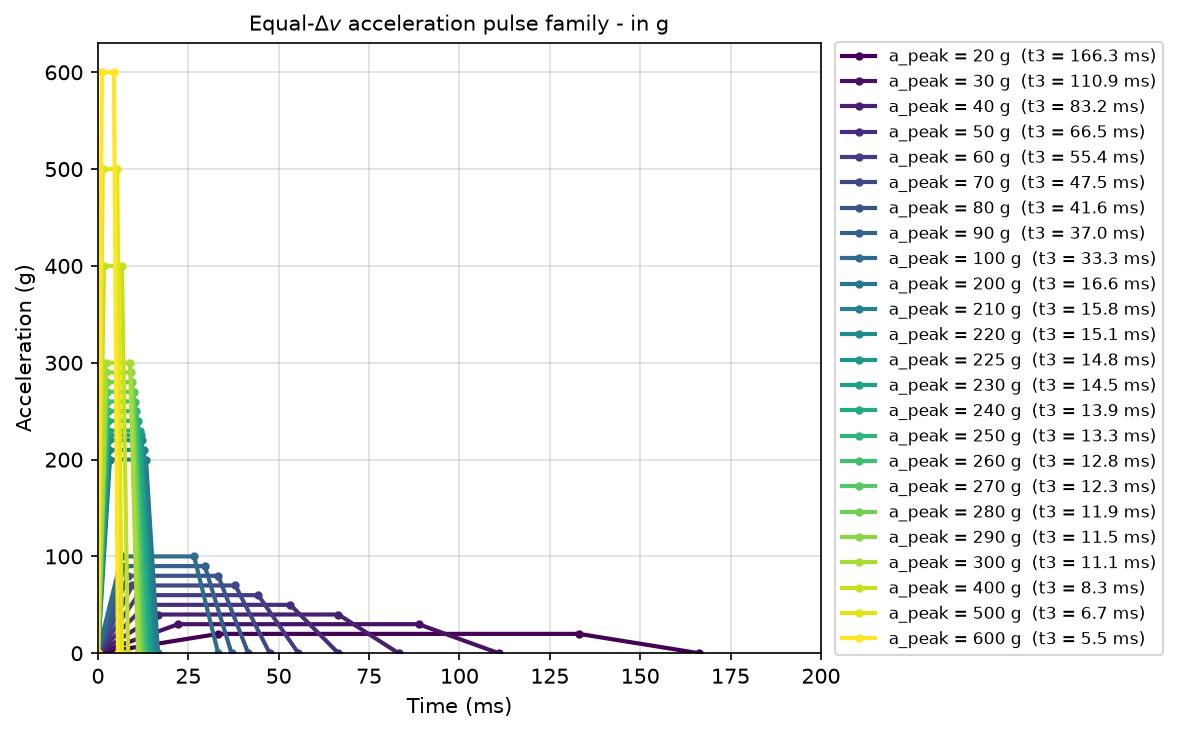
\includegraphics[width=0.8\textwidth]{figures/chap4/step3-fem-sled/accel_curve_family_g.png}
    \caption{Family of trapezoidal acceleration pulses with equal area $\lVert \mathbf{u}_0 \rVert$: a higher plateau amplitude $a$ corresponds to a shorter plateau duration $t_p$.}
    \label{fig:accel-pulses}
\end{figure}

The maximum acceleration (the value of the acceleration plateau) that the phials can withstand is found with a search procedure analogous to the calibration of \texttt{FT} for Step 2 of the workflow: the amplitude $a$ is varied step by step, with the duration of the simulation adjusted through \cref{eq:pulse_area}, until the threshold for the initiation of phial failure is found. Since a larger amplitude also implies a shorter pulse, the resulting limit refers to this pulse shape and to the given initial velocity and is expressed in terms of the acceleration prescribed at the rings. 


\subsubsection{Mass scaling}
% where it is applied, added mass (%), resulting dt gain
% effect on phial inertial load; correction or sensitivity check

Explicit analyses must abide to the Courant-Friedrichs-Lewy (CFL) condition, which limits the possible timestep amplitude $\Delta t$ adopted in the calculation due to numerical stability constraints. Specifically, the condition is based on the most critical combination of two factors, shown in the following equation:

\begin{equation}\label{eq:t-crit-expl}
    \Delta t \le \Delta t_{\text{crit}} = \frac{L_e}{c}
\end{equation}

\noindent where:
\begin{itemize}
    \item $L_e$ is the characteristic length of the critical element in the model (e.g., shortest side or minimum height of a shell or solid element);
    \item $c$ is the acoustic wave speed (speed of sound) in the material of that element.
\end{itemize}

The element-specific combination of $L_e$ and $c$ that minimises their ratio dictates the size of the allowable timestep and, therefore, the speed at which the calculations can continue. In the case of the sled test model, the 0.1\,mm phial shells set the stable timestep ($\Delta t \approx l_e/c \approx 1.9\times10^{-5}$~ms), yielding $10^6$ to $10^7$ calculation cycles for phenomena of the duration between 10 and 100\,ms such as the simulated event, demanding significant computational capacity and runtime.

As the speed of sound in elastic materials is inversely proportional to the square root of the material's density ($c = \sqrt{\frac{M}{\rho}}$, where $M$ represents the appropriate elastic modulus, such as Young's modulus $E$ or bulk/shear moduli $K$ and $G$), a common procedure adopted in FEM practice to raise the stable timestep is to locally increase material density in the critical elements by artificially adding non-physical mass, directly reducing $c$ and subsequently increasing $\Delta t_{\text{crit}}$ as per \cref{eq:t-crit-expl}. In LS-DYNA, \textit{mass scaling} is activated through the keyword \kw{CONTROL\_TIMESTEP}, parameter \texttt{DT2MS}: given the target $\Delta t$, and choosing whether scaling applies only to elements below the target (negative \texttt{DT2MS}), the solver calculates the density increase and, therefore, the local non-physical mass increase to bring the stable timestep up to the hard-coded value. While mass scaling accelerates solver runtime, excessive artificial mass addition might compromise physical realism of the simulated phenomenon. While this is negligible in static or quasi-static conditions where dynamic effects do not influence numerical results, it becomes particularly relevant during dynamic impact events, where the inertial component significantly dictates stress magnitudes and transient structural responses. An ideal timestep to impose is one that minimises calculation runtimes while keeping the model's physics realistic and the numerical results reliable.

Due to the glass phials' fine mesh, artificial mass is added entirely on the phial. Through a process of trial-and-error, it was observed that increasing the timestep by one order of magnitude would result in a $\approx$50 to 60x local mass increase, which in turn would reduce the phial's fundamental frequency by a factor of $\sqrt{[50,\,60]} \approx [7.1,\,7.7]\times$ (considering the relation $\omega_1 = \sqrt{\frac{k}{m}}$, where \textit{k} and \textit{m} are the equivalent stiffness and mass of a mass-spring system representing the payload assembly). In transient impact dynamics, reducing the natural frequency shifts the system more out of phase with the input pulse width, artificially smoothing or delaying the peak contact forces between the phial and the sponge. To avoid incurring in this possibility, it was decided to settle for a timestep value of $2\times10^{-5}$\,ms, increasing the phial's mass only by $2.7\times10^{-4}$\,g and, thus, maintaining overall reliability.


\subsubsection{Requested outputs and failure detection}
Numerically, an event counting as a failure of the glass phial corresponds to observing the \texttt{MAT\_GLASS} \textit{Extra History Variable \#1} \texttt{HISV\#1} $\geq 1$, meaning that a crack is initiated with the failure of \texttt{NIPF} $= 5$ thickness integration point. Verification of crack formation can be observed in the results (\texttt{d3plot}) file activating the \texttt{HISV\#1} contour plot and using the max-IP fringe. 

The failure event must be comparable to the one produced experimentally in Step 1, i.e. a similar failure mode should be observed in the sled test simulation to guarantee the reliability of the observed allowable acceleration. The allowable is therefore taken as the highest acceleration level without failure, which lies within the bracket between the last pass and the first fail, whose width equals the sweep step and is stated in the results section below.


\subsection{Results}
\subsubsection{Failure location and mode} % crack origin vs Step 2 / MTS breaking modes
Dilemma between choosing similar failure mode and similar loading scenario, loading scenario is less conservative (higher acceleration allowable) so I went with similar failure mode although caused by different loading scenario. 

\begin{figure}[h!]
    \centering
    % TODO: replace the placeholder box with the actual figure once available
    % \includegraphics[width=0.8\textwidth]{figures/chap4/step3-fem-sled/phial_damage_hisv1.png}
    \fbox{\parbox[c][6cm][c]{0.8\textwidth}{\centering Figure placeholder: phial damage, \texttt{HISV\#1} contour}}
    \caption{Glass phial damage in the sled test simulation: \texttt{MAT\_GLASS} \texttt{HISV\#1} contour plot (max-IP fringe), where \texttt{HISV\#1} $= 1$ marks crack initiation.}
    \label{fig:step3-phial-damage-hisv1}
\end{figure}



\subsubsection{Model verification}        % energy balance, added mass, hourglass
Phial internal-energy discontinuity (\texttt{MATSUM}), plus the jump in the phial node's acceleration (\texttt{NODOUT}).

----> HOW???? rethink this

\subsubsection{Acceleration sweep}        % survive/fail per level -> allowable
* manually verified, when history variable turns into 1!!!
* tolerance -> 5 g's



\subsubsection{Step 3 deliverable: allowable payload acceleration}
* allowable value: XXX (mabe 230 g)
* main failure mode: dome breaking
* impact direction : perpendicular to axial

\begin{table}[h!]
\centering
\caption{Allowable payload acceleration obtained from the sled test simulation.}
\label{tab:step3-summary-data}
\begin{thesistable}{
  colspec = {X[1.3,l] X[1,l] X[1.6,l]},
}
Quantity & Value & Source / note \\
Allowable peak acceleration ($a_{allow}$) & \hl{230}\,g & Highest plateau amplitude without phial failure; bracket width equal to the sweep step of \hl{10}\,g \\
Critical loading direction & Perpendicular to the phial axis & Most critical degree of freedom of the X/Y/Z sweep \\
Main failure mode & Dome breaking & Comparable to Mode A of Step 1 (\cref{tab:step1-summary-data}) \\
Velocity shed ($\lVert \mathbf{u}_0 \rVert$) & \qty{26.1}{\metre\per\second} & Resultant of $u_{x0}$ and $u_{y0}$ from Step 0 (\cref{tab:step0-summary-data}) \\
Pulse shape & Trapezoidal & \texttt{RISE\_FRACTION} = 0.2, area constrained by \cref{eq:pulse_area} \\
\end{thesistable}
\end{table}


